\documentclass[conference]{IEEEtran}
\usepackage{cite}
\usepackage{amsmath,amssymb,amsfonts}
\usepackage{algorithmic}
\usepackage{graphicx}
\usepackage{textcomp}
\usepackage{xcolor}
\usepackage{array}
\usepackage[caption=false,font=normalsize,labelfont=sf,textfont=sf]{subfig}
\usepackage{stfloats}
\usepackage{tabularx}
\usepackage{booktabs}
\def\BibTeX{{\rm B\kern-.05em{\sc i\kern-.025em b}\kern-.08em
    T\kern-.1667em\lower.7ex\hbox{E}\kern-.125emX}}
\begin{document}

\title{An Image-Based Imitation Learning Framework \\ for Robotic Writing Task}
\author{\IEEEauthorblockN{1\textsuperscript{st} Wenjin Xu}
\IEEEauthorblockA{\textit{College of Automation Science and Engineering} \\
\textit{South China University of Technology}\\
Guangzhou, China \\
202320116672@mail.scut.edu.cn}
\and
\IEEEauthorblockN{2\textsuperscript{nd} Chenguang Yang}
\IEEEauthorblockA{\textit{College of Automation Science and Engineering} \\
\textit{South China University of Technology}\\
Guangzhou, China \\
cyang@ieee.org}
}
\maketitle
\begin{abstract}
This paper presents an image-based imitation learning framework that enables robots to acquire writing skills, particularly for traditional Chinese calligraphy. The framework encodes the temporal information of static images, transforming them into a dynamic format suitable for dynamic system demonstration methods. A deviation analysis method is proposed to enhance the learning of stroke thickness. Furthermore, the framework allows skill generalization across different writing environments and paper sizes. The effectiveness of the proposed framework is validated through simulations and real-world experiments.
\end{abstract}

\begin{IEEEkeywords}
Imitation Learning, Computer Vision, Gaussian Mixture Model, Dynamic Movement Primitive, Chinese Calligraphy
\end{IEEEkeywords}

\section{Introduction}
Today, the technology is rapidly evolving and undergoing swift generational changes. New technologies, represented by robotics, are continuously transforming people's lives. In the past, robots were limited to performing simple and repetitive tasks within the confines of factories. However, with the development of human-robot skill transfer, robots can not only streamline production tasks but also increasingly serve humanity in everyday life. There has been some research concerning the transfer of writing skills between humans and robots, mainly learning from human demonstration (LfD), also known as imitation learning. Imitation learning primarily encompasses three main approaches: teleoperation-based demonstration, kinesthetic demonstration and visual-based demonstration. The teleoperation-based demonstration allows humans to transfer skills by manipulating a teleoperation device\cite{Lu2024}. However, due to the significant differences between the teleoperation joystick and the writing tools commonly used by humans, the transfer of writing skills is not effective and natural. Kinesthetic demonstration primarily involves dragging the robot's end-effector through manual manipulation and recording the robot's motion to transfer the skill\cite{Dong2023a}. This method has the same problem: not intuitive and does not conform to the natural writing habits of humans. 

Inspired by the human process of learning, the visual-based demonstration is a better way for skill transfer. In \cite{Zhang2019}, a system based on CNN has been developed to learn traditional Chinese calligraphy skills. The network is utilized to construct a calligraphy skill calligraphy database and the system incorporates a digitizing tablet to collect handwriting data, which means a considerable amount of demonstration work is required. In \cite{Mees2020}, the Adversarial Skill Networks (ASN) is presented, which can learn skills from the video. However, for writing tasks, the limited availability of suitable writing skill videos poses a challenge for large-scale training. In contrast, the amount of suitable writing images is much larger. It is more viable to learn writing skills from images directly.

In \cite{Zhang2023}, the author proposes a method which can directly learn writing skills from images of English letters. In \cite{Li2021, Li2022, Li2024}, the proposed method can learn from images of modern Chinese calligraphy. Both of them are based on the eight-neighbour method for extracting the skeleton to obtain the demonstration trajectory, and generalizing by Dynamic Movement Primitives (DMP)\cite{Ijspeert2013}. However, they can only learn the motion patterns from the demonstration images, unable to capture the deeper features, like the thickness of the strokes. In \cite{Yang2019}, the integration with the Gaussian Mixture Model (GMM) expands the learning capabilities of the DMP, enabling it to learn multiple demonstrations simultaneously. In \cite{Yang2019c}, the improvement of the Fuzzy Gaussian Mixture Model (FGMM)\cite{Ju2012} enhance the learning effect. These methods are capable of learning the deviation among multiple demonstrations, but they are still insufficient for writing tasks that demand high precision in stroke thickness, like traditional Chinese calligraphy. In this paper, we propose an image-based imitation learning framework for robotic writing tasks, especially for the writing task of traditional Chinese calligraphy. The main contributions of this article are listed as follows:

1) A novel imitation learning framework is proposed which can transfer the writing skill to the robot through an image. The static data is transformed into a dynamic format, allowing us to employ the demonstration methods that are exclusive to dynamic systems.

2) We propose a learning method which can not only learn the trajectory from multiple demonstrations but also learn the deviation among them. In the writing task, it can be used to learn the thickness of strokes.

3) We propose a DMP-based method for the generalization of writing skills, particularly for traditional Chinese calligraphy. The framework is capable of adjusting the reproduction on different sizes of paper.

\section{Preliminaries}
\subsection{Fuzzy Gaussian Mixture Model}
\begin{figure*}[!t]
    \centering
    \subfloat[]{
    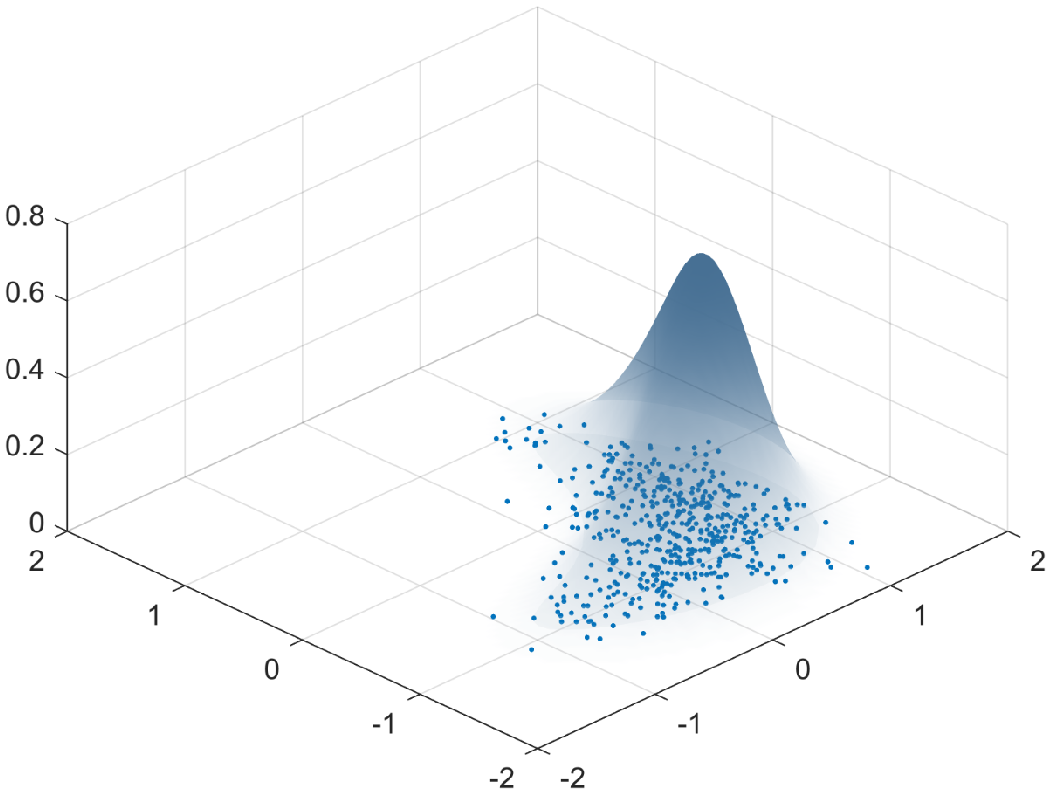
\includegraphics[width=2in]{./fig/fig2-a.pdf}
    }
    \subfloat[]{
        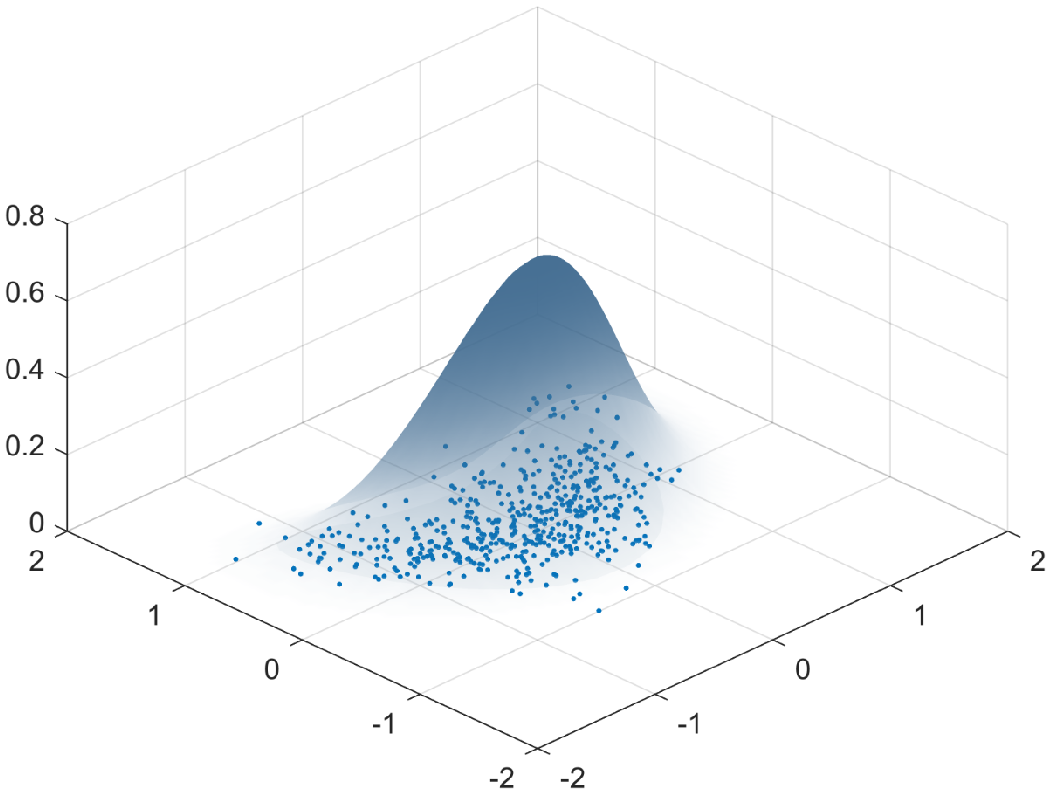
\includegraphics[width=2in]{./fig/fig2-b.pdf}
    }
    % \subfloat[]{
    % 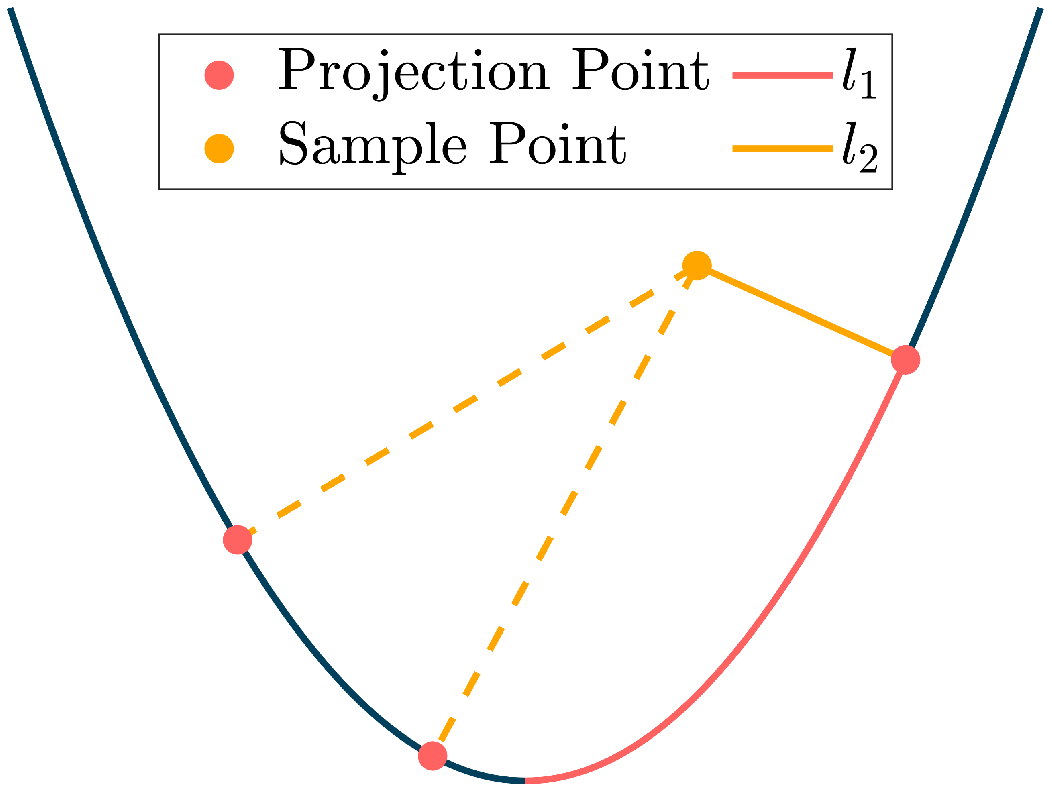
\includegraphics[width=1.5in]{./fig/fig2-c.pdf}
    % }
    \subfloat[]{
        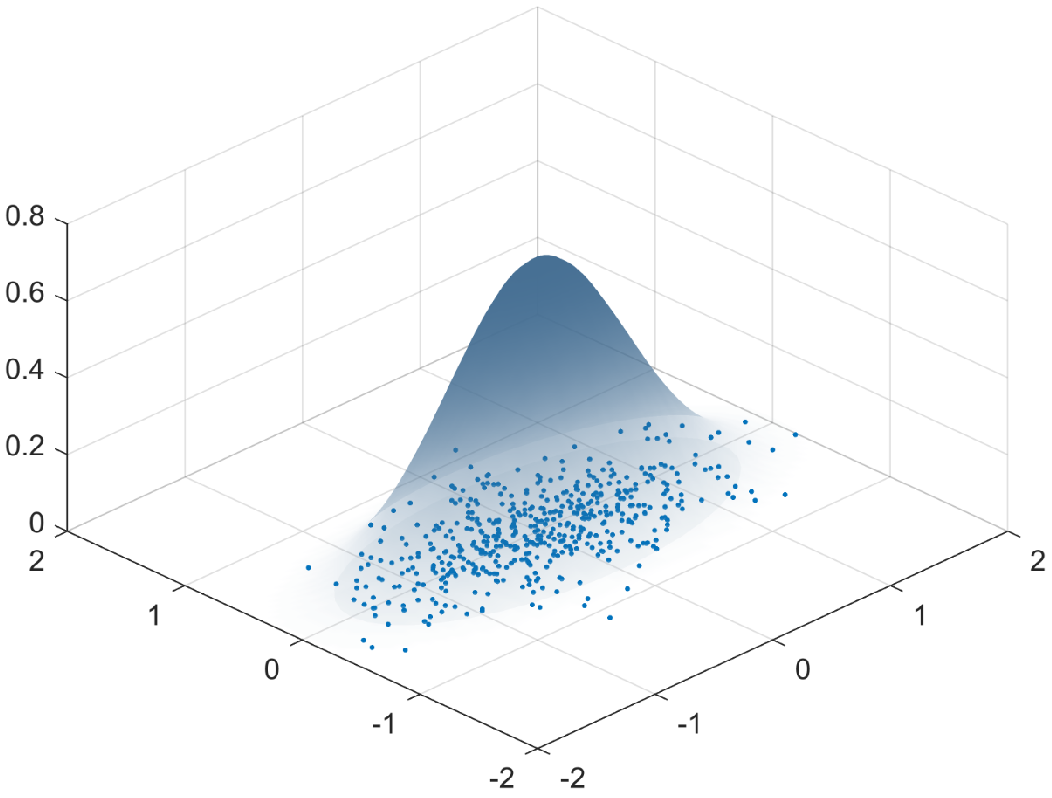
\includegraphics[width=2in]{./fig/fig2-d.pdf}
    }
    \caption{The data transformation process of FGMM. (a) Original Samples (b) Transformed Samples (c) Projected Samples}
    \label{fig2}
\end{figure*}
GMM has been widely applied in various fitting scenarios\cite{Chen2020a, Chen2021a, Mei2023}. Paper \cite{Ju2012} introduce a modified GMM called the FGMM. It combines the conventional GMM with Active curve axis Gaussian mixture models (AcaG)\cite{Zhang2005} and introduces a dissimilarity function to accelerate convergence. Fig.\ref{fig2} represents the data transformation process of FGMM. First, the k-means algorithm divides the dataset into $K$ classes. For each class of data, we transfer them to a new coordinate through Principal Component Analysis (PCA):
\begin{equation}
    Y_i=Q_i \times (X_i-T_i)
\end{equation}
where $Q_i$ and $T_i$ denote the rotation matrix and translation vectors. $X_i$ is data which belongs to the $i^{th}$ components, as Fig.\ref{fig2}(a) presents. The transformed data $Y_i$ presented in Fig.\ref{fig2}(b) have zero mean, and their principal axis aligns with the transformed x-axis. All data are assumed as two-dimensional in this paper. The Least-Squares Fitting Method (LSFM) is used to fit the data using a parabolic curve. The projection points on the parabolic curve are used to replace the sample points for calculating the posterior probability. A sample may have multiple projection points with the shortest distance. Then we calculate the arc length of the $j^{th}$ projection points $\{z_{1j},z_{2j}\}$:
\begin{equation}
    l_{1j}=\int_{(0,b)}^{(z_{1j},z_{2j})}\sqrt{(dz_{1j})^2+(dz_{2j})^2}
\end{equation}

And the distance between $x_t$ and $z_j$ is:
\begin{equation}
    l_{2j}=\sqrt{(x_{1t}-z_{1j})^2+(x_{2t}-z_{2j})^2}
\end{equation}

The expected projected points are calculated using the probability in a zero-mean Gaussian model as weights:
\begin{equation}    L_{sn}=\frac{\sum^{J_{in}}_{j=1}p(l^i_{sj}|0,\Sigma^{old}_{si})l^i_{sj}}{\sum^{J_{in}}_{j=1}p(l^i_{sj}|0,\Sigma^{old}_{si})}~(s=1,2)
\end{equation}
where Fig\ref{fig2}(c) illustrates the distribution of the projected samples. The modified EM algorithm is proposed to estimate the parameters of FGMM. FGMM introduces the Fuzzy C-means mechanism to accelerate the convergence speed of the EM algorithm.

\subsection{Dynamic Movement Primitive}
DMP is an LfD model based on dynamic systems and is capable of skills generalization\cite{Ijspeert2013}. It is widely used in various imitation learning systems\cite{Zhang2020, Luo2023}. It consists of a second-order dynamic system and a non-linear function, allowing it to encode motion trajectories with fewer parameters while maintaining stability:
\begin{equation}
    \tau^2 \ddot y = \alpha(\beta(g-y)-\tau \dot y) + f
    \label{eq4}
\end{equation}
where the parameter $\beta = \alpha / 4$, in order to avoid overshooting and ensure stable convergence. To decouple the non-linear equation from time, a canonical system $x(t)$ is used to drive the dynamic system:
\begin{equation}
    \tau \dot x = - \kappa x
\end{equation}

The second term $f$ is a non-linear function that controls the intermediate convergence process. The non-linear function $f$ can be expressed as:
\begin{equation}
    f(x)=\frac{\sum\limits_{i=1}^{N} \Psi_{i}(x) w_{i}}{\sum\limits_{i=1}^{N} \Psi_{i}(x)}x(t)(g-y)
    \label{eq5}
\end{equation}
where, $\Psi(t)$ is a Radial Basis Function (RBF), expressed as:
\begin{equation}
    \Psi_i(x)= \exp \left(-\frac{\left(x-\mu_i \right)^{2}}{2 \sigma_i^{2}}\right)
\end{equation}
where $N$ represents the number of RBF, $\mu_i$ represents the position of the $i^{th}$ basis function, and $\sigma_i$ represents the width of the $i^{th}$ basis function. $\omega_i$ represents the weight of the $i^{th}$ radial basis function, which needs to be obtained by learning from the demonstration trajectory $y_{dms}$. $f_{dms}$ can be expressed as:
\begin{equation}
    f_{dms} = \tau^2 \ddot y_{dms} - \alpha(\beta (g-y_{dms})-\tau \dot y_{dms})
    \label{eq6}
\end{equation}
where Locally Weighted Regression (LWR) is used to determine the weight parameter $w_{i}$, which can control the $f(x)$ to fit $f_{dms}$.

\section{Methodology}
\subsection{System Description}
\begin{figure*}[!t]
    \centering
    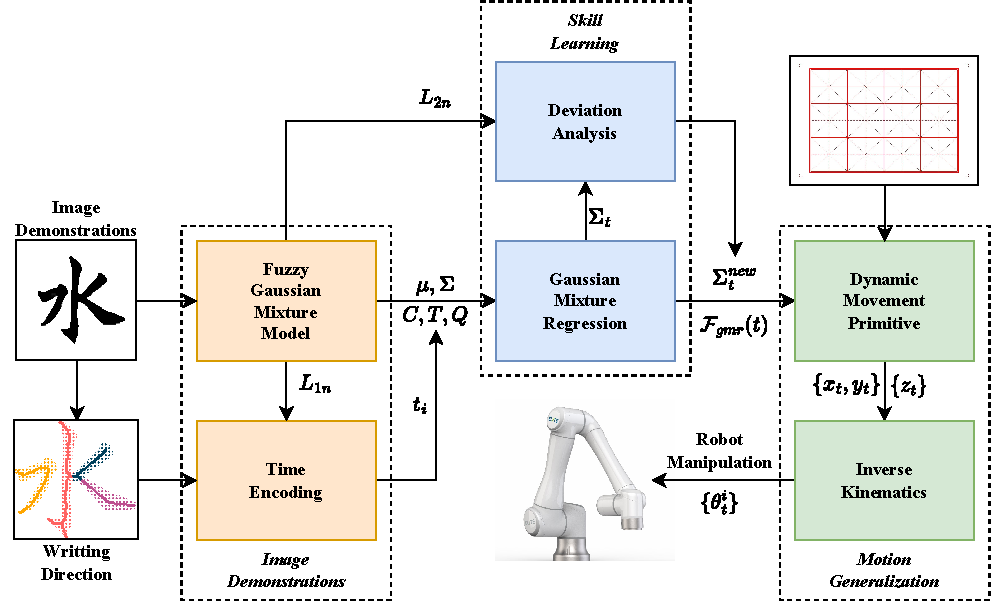
\includegraphics[width=6.2in]{./fig/fig1a.pdf}
    \caption{The block diagram of the proposed framework. The framework contains three aspects. The framework input is the image written by the human, and the output is the motion sequence of the robot.}
    \label{fig1}
\end{figure*}
The block diagram presented in Fig.\ref{fig1} illustrates the framework of the imitation learning system for robotic handwriting tasks. The system can learn writing skills from images, particularly focusing on the deviation information within them, and ultimately achieving skill generalization in various environments. The entire system encompasses three aspects:

1)~Image Demonstration: The demonstration part transfers the writing skill to the robot through the character image written by a human. The proposed framework enables robot learning parameters of FGMM from a static image. 

2)~Skill Learning: With the parameters estimated in the previous part, the writing skills can be encoded by Gaussian Mixture Regression (GMR). The normal GMR method can generate the trajectory very well. However, the effect of learning the deviation among samples is not that good. We proposed a novel approach called deviation analysis to enhance the deviation learning ability of GMR.

3)~Motion Generalization: It is common to adjust the generalization effect of writing skills in different situations, like changing the size of the written font to adapt the various types of papers in the real world. DMP is used to make the skill have great generalization performance.

\subsection{Time Encoding}
Traditional vision-based demonstrations are mostly obtained by recording motion sequences to acquire demonstration trajectories. Data usually contains time sequences, and time-driven methods like GMR and DMP are used for motion encoding and skill learning. However, in some scenarios, the time sequence of demonstration trajectories is missing, like demonstrating writing skills through an image. A new method based on FGMM is proposed for encoding the time series of demonstration trajectories.

First, estimate the parameter of FGMM using the EM algorithm proposed before. Here we use a Chinese character stroke image as an example, presented in Fig.\ref{fig3}. The direction is needed to determine a general direction of movement, which does not need to be very precise. Each sample has a transformed point $L_n$ after a non-linear transformation during the parameter estimation. For most writing tasks involving movement along the principal axis, time information can be obtained through $L_{1n}$, which denotes the relative position of the sample on the principal axis. First we transfer the transformed sample from the first component $L_{1}^{(1)}=\{L_{11}^{(1)}, \hdots, L_{1n}^{(1)}\}$ to a zero starting point:
\begin{equation}
    t^{(1)}=\{L_{11}^{(1)}, \hdots, L_{1n}^{(1)}\}-min(L_{1}^{(1)})
\end{equation}

For the second component of transformed sample $L_{1}^{(2)}$, transfer them to the end of the first sequence:
\begin{equation}
    t^{(2)}=\{L_{11}^{(2)}, \hdots, L_{1n}^{(2)}\}-min(L_{1}^{(2)})+max(L_{1}^{(1)})
\end{equation}
if there are multiple components, repeat this process until the end. The time sequence is denoted as $\{t^{(1)},t^{(2)},\hdots,t^{(i)}\}$. Fig.\ref{fig4} presents the result of time encoding. The arrow on the sample point indicates the direction of time flow.
\begin{figure}[!t]
    \centering
    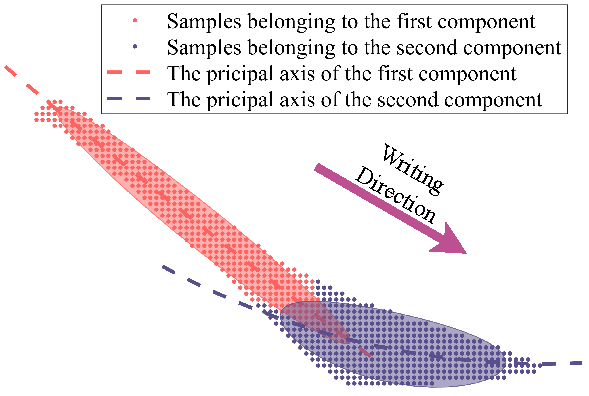
\includegraphics[width=3in]{./fig/fig3.pdf}
    \caption{Fitting Chinese stroke using FGMM.}
    \label{fig3}
\end{figure}

\begin{figure}[!t]
    \centering
    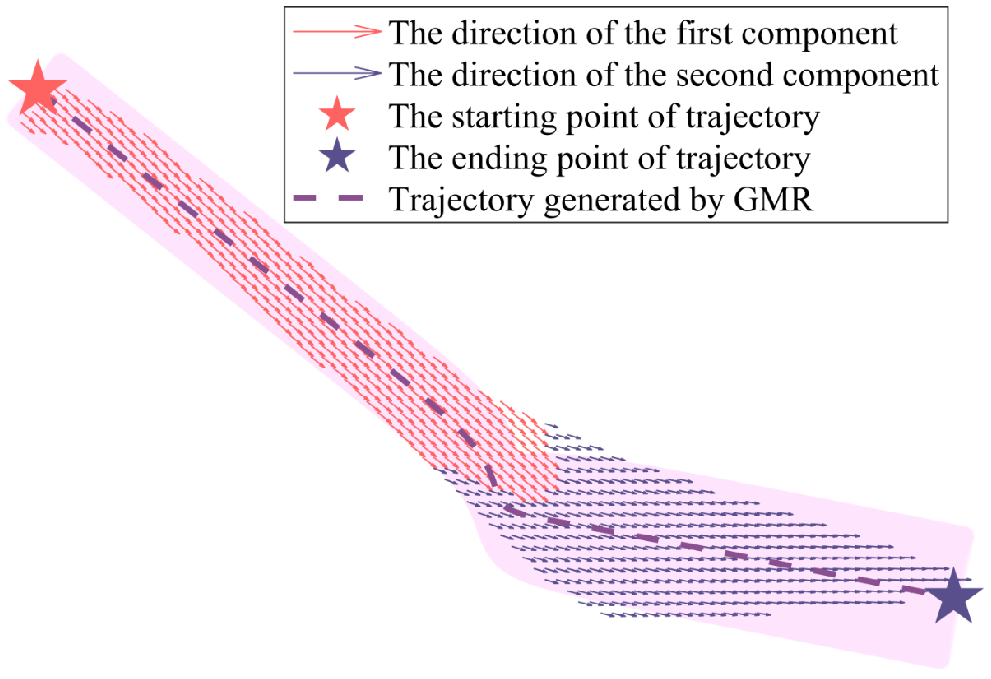
\includegraphics[width=3in]{./fig/fig4.pdf}
    \caption{The result of time encoding and GMR.}
    \label{fig4}
\end{figure}

After time encoding, the time-driven method can be used for motion planning in writing tasks. Gaussian Mixture Regression (GMR) is a statistical learning technique that combines the GMM with linear regression. The regression function can be considered as obtaining the expectation of an event for the output $X$ conditional on the input $t$:
\begin{equation}
    \mathcal{F} _{gmr}(t)=E(X|t)
\end{equation}

Assume that $X$ and $t$ follow the Gaussian distribution, the event satisfies:
\begin{equation}
    X|t \sim G(\mu_X+\frac{\sigma_{21}}{\sigma_{1}}(t-\mu_t),\sigma_{2}-\frac{\sigma_{12}\sigma_{21}}{\sigma_{1}})
\end{equation}
where $\sigma_{1}$ and $\sigma_{2}$ denote the variance of $t$ and $X$, $\sigma_{12}$ and $\sigma_{21}$ denote the covariance between $t$ and $X$. Consider that the Gaussian mixture model can be seen as a linear combination of Gaussian distributions, the expectation can be written as:
\begin{equation}
    \mathcal{F} _{gmr}(t)=\sum\limits_{i=1}^{K}w_i(t)\eta_i(t)
\end{equation}
where
\begin{equation}
    w_i(t)=\frac{\alpha_{i}G(t|\mu_{i}(t),\sigma_{it})}{\sum_{i=1}^{K}\alpha_{i}G(t|\mu_{i}(t),\sigma_{it})}
\end{equation}
\begin{equation}
    \eta_i(t)=\mu_{iX}+\frac{\sigma_{21i}}{\sigma_{1i}}(t-\mu_{it})
    \label{eq2}
\end{equation}

\subsection{Deviation Analysis}
In some scenarios like transferring writing skills to robots, the robot needs to learn not only the trajectory information of samples but also the deviation among them. The pink area shown in Fig.\ref{fig4} denotes the covariance of trajectory generated by GMR. The fitting effect is not ideal. A new method based on FGMM is proposed, which is called Deviation Analysis (DA). Analyse the deviation of samples to generate a variance sequence for a better fitting effect. In addition to generating a trajectory from time input, GMR can also generate a corresponding covariance sequence $\{\Sigma_1,\hdots,\Sigma_t\}$. It denotes the covariance among samples in time $t$. The covariance matrix implicitly contains the posture and deviation of the trajectory. They can be obtained by eigenvalue decomposition:
\begin{equation}
    \Sigma_t=R_tD_tR_t^{-1}
\end{equation}
where $D_t$ and $R_t$ represent the eigenvalues and eigenvectors of the covariance matrix, respectively. According to the geometric meaning of eigenvalue decomposition, they also represent the scaling effect and rotation effect of the covariance matrix, respectively, which represent the deviation and posture information of the trajectory. $L_{2n}$ defines the distance between the transformed sample and the principal axis. It can be used to define a new scaling matrix. According to the $3\sigma$ rule, the new scaling matrix is defined as:
\begin{equation}
    D_t^{new}=\left[
        \begin{array}{cc}
            (\frac{1}{3}L_{2t})^2 & 0       \\
            0                     & D_{22t}
        \end{array}
        \right]
    \label{eq3}
\end{equation}
the new covariance sequence is:
\begin{equation}
    \Sigma^{new}_t=R_tD^{new}_tR_t^{-1}
\end{equation}

\section{Experiments}
\subsection{Simulation}
In this part, The proposed method is verified through simulation. A Chinese calligraphy image is used as the demonstration image, denoted in Fig.\ref{fig1}. Paper \cite{Li2022} propose an observation-based algorithm which can extract strokes from the Chinese character image, as Fig.\ref{fig1} represents, and denotes their direction, which can determine the order of GMM components, as Fig.\ref{fig5}(a) and (b) denote. Fig.\ref{fig5}(a) and (b) also show the result of fitting the Chinese character image by conventional GMM and FGMM, respectively. The conventional GMM need to use 8 components to fit the character well. In contrast, the FGMM only requires 7 components. The following three methods will be compared to the effect of writing tasks: the GMM without DA, the GMM with DA and the FGMM with DA. To maintain the accuracy of the comparison, the writing tasks are simulated based on a unified method. Assume the discrete trajectory is $\{(x_1,y_1),\hdots,(x_N,y_N)\}$, and the covariance matrix sequence is $\{\Sigma_1,\hdots,\Sigma_N\}$. At time t, the writing trajectory is defined as:
\begin{equation}
    o_t =[cos(p),sin(p)]\sqrt{3\Sigma_t}+[x_t,y_t]~~(-\pi<p<\pi)
\end{equation}
where the area represented by $o_t$ indicates the writing trace at time t. The writing simulation results for the three methods are denoted in Fig.\ref{fig5}(c)-(e).
\begin{figure}[!t]
    \centering
    \subfloat[]{
        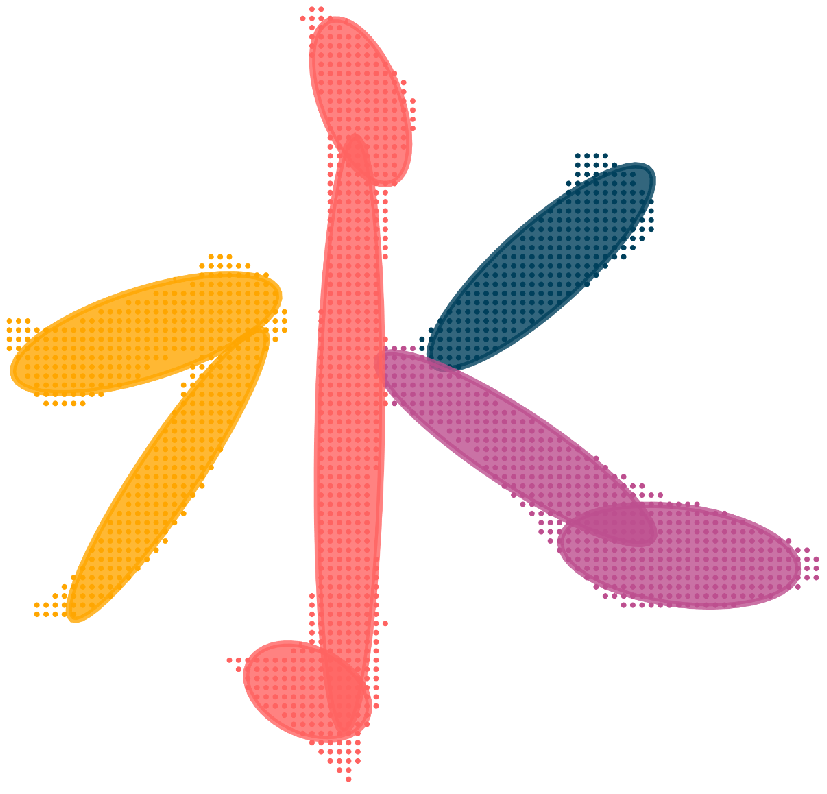
\includegraphics[width=1.5in]{./fig/fig5-b.pdf}
    }
    \subfloat[]{
        
\includegraphics[width=1.5in]{./fig/fig5-c.pdf}
    }
    \quad
    \subfloat[]{
        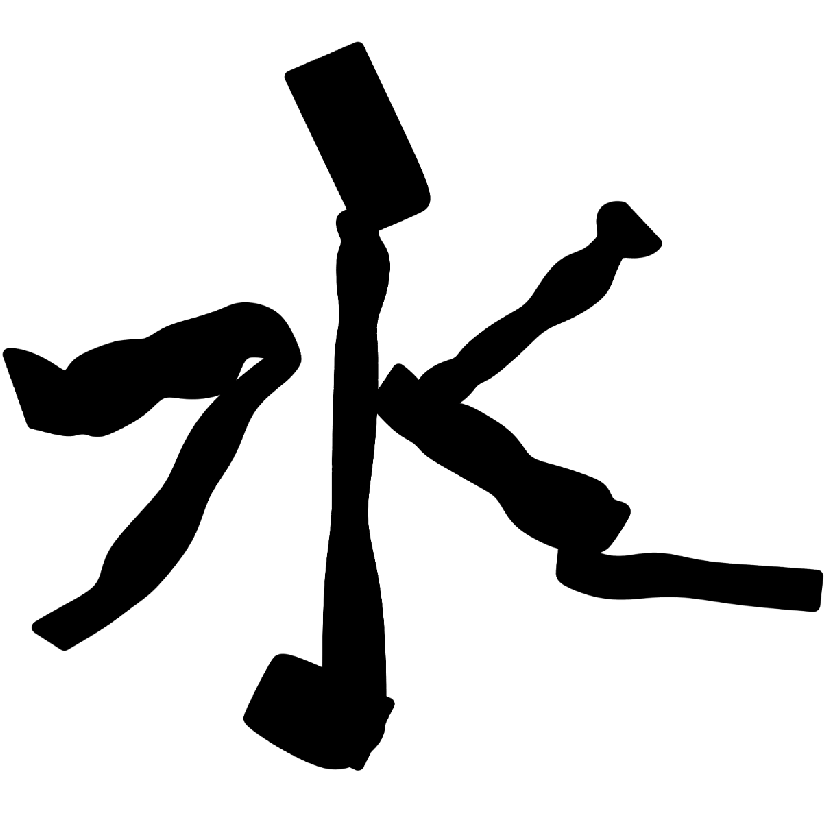
\includegraphics[width=1in]{./fig/fig5-d.pdf}
    }
    \subfloat[]{
        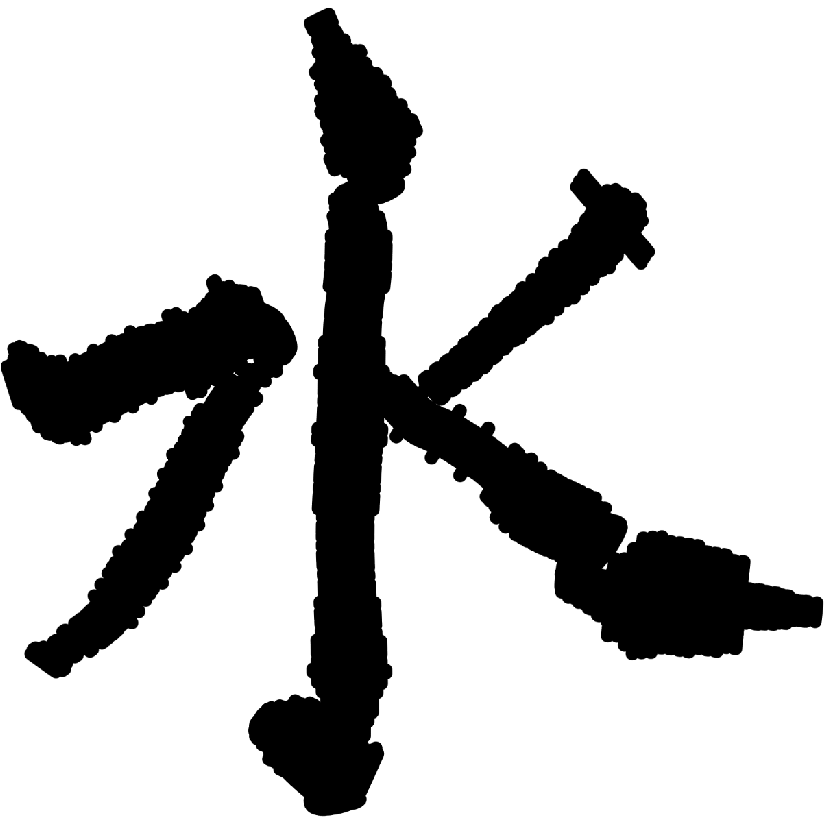
\includegraphics[width=1in]{./fig/fig5-e.pdf}
    }
    \subfloat[]{
        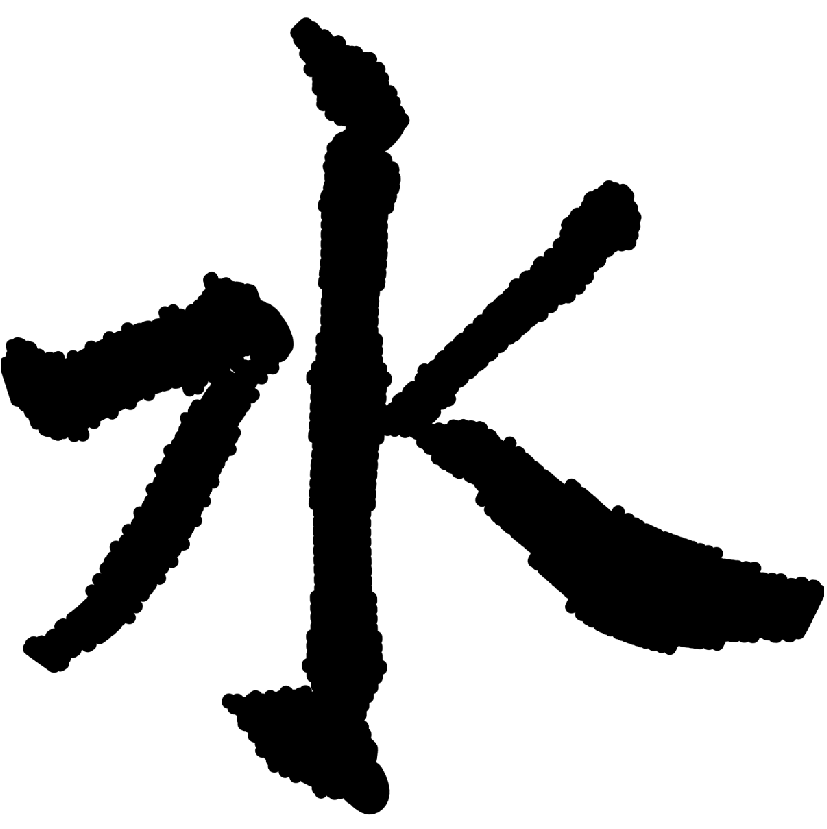
\includegraphics[width=1in]{./fig/fig5-f.pdf}
    }
    \caption{The writing simulation of Chinese character "water". (a) Fitting Chinese character using GMM (b) Fitting Chinese character using FGMM (c) Simulation result of the GMM method (d) Simulation result of the GMM+DA method (e) Simulation result of the FGMM+DA method.}
    \label{fig5}
\end{figure}



\begin{table}[!t]
    \centering  
    \caption{THE IQA RESULT OF THE SIMULATION}
    \label{tab2}
    \begin{tabular}{cccc}
    \toprule
    Metric & GMM & GMM+DA & \textbf{FGMM+DA} \\
    \midrule
    PSNR$\uparrow$ & 10.7447 & 11.5709 & \textbf{12.1143} \\
    FSIM$\uparrow$ & 0.7896 & 0.7901 & \textbf{0.7990} \\
    SSIM$\uparrow$ & 0.7867 & 0.7928 & \textbf{0.8019} \\
    VSI$\uparrow$ & 0.7665 & 0.8018 & \textbf{0.8126} \\
    VIF$\uparrow$ & 0.0203 & 0.0225 & \textbf{0.0236} \\
    IFC$\uparrow$ & 0.0452 & 0.0493 & \textbf{0.0514} \\
    VOI$\downarrow$ & 2.9374 & 2.8622 & \textbf{2.8019} \\
    MSE$\downarrow$ & 5477.8718 & 4528.9159 & \textbf{3996.2290} \\
    DISTS$\downarrow$ & 0.3535 & 0.3522 & \textbf{0.3463} \\
    LPIPS$\downarrow$ & 0.3354 & 0.3058 & \textbf{0.2951} \\
    \bottomrule
    \end{tabular}
\end{table}

To compare the fitting effect of the simulation results with the demonstration image, we introduce 10 commonly used Image Quality Assessment (IQA) methods as evaluation metrics. They are all Full Reference (FR) methods, which can evaluate the differences between the simulation results and the demonstration image. The evaluation results are presented in Table.\ref{tab2}. Both FGMM and DA enhance the writing results a lot. Then, we verify the generalization performance of the method. Assuming the paper size for reproducing the writing skills is half the size of the demonstration image, the starting and ending points of the Chinese character strokes need to be re-determined. Here, the one-point perspective is used to determine the new starting and ending points. Then the proposed framework can reproduce the writing skills to fit this new scenario. The reproduction trajectories and their starting and ending points are represented in Fig.\ref{fig7}.
\begin{figure}[!t]
    \centering
    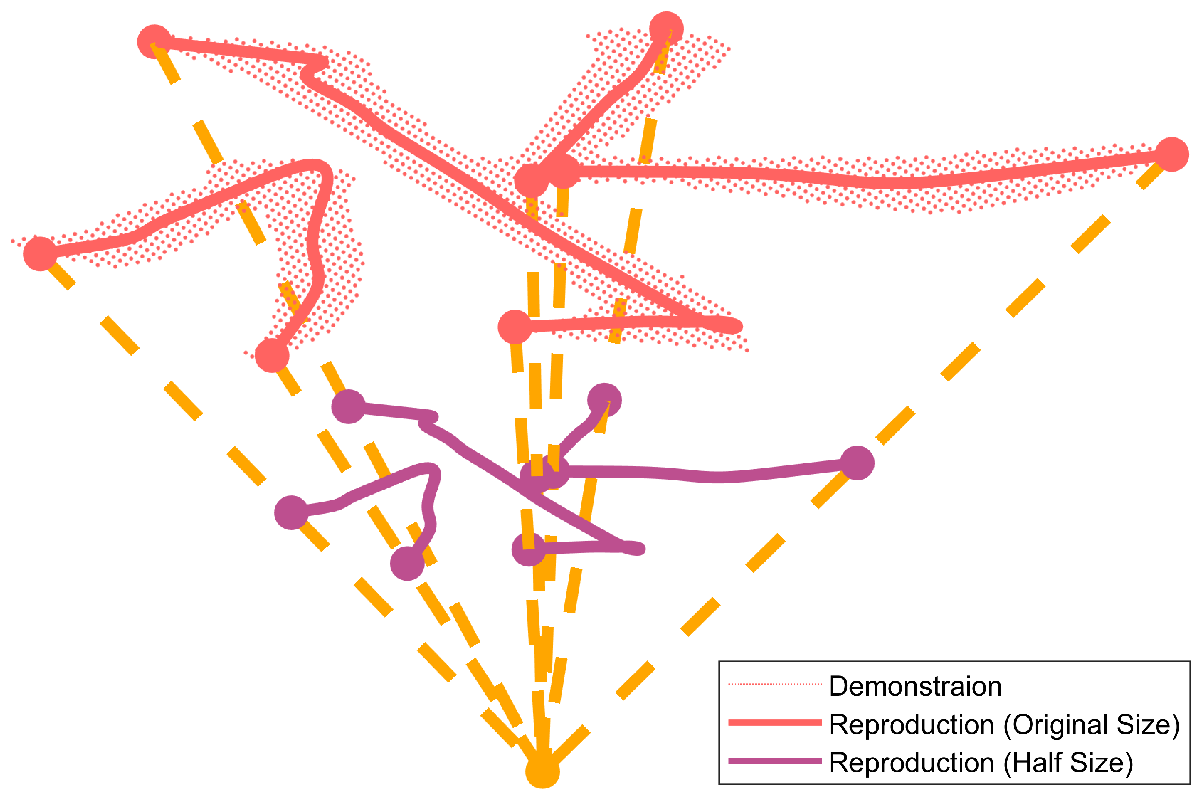
\includegraphics[width=3in]{./fig/fig7.pdf}
    \caption{The new starting and ending points for each stroke are determined by the one-point perspective. And the reproduction of writing skills for the whole Chinese character in two sizes: the original size and the half size.}
    \label{fig7}
\end{figure}

\subsection{Real-World Experiment}
In this part, we conducted a real-world experiment to validate the effectiveness of the proposed method on the platform represented in Fig.\ref{fig8}(a). The platform contains a webcam and the EC66 robot, which are used to capture the demonstration image and execute the writing skills learnt before. We employed the brush pen as the end-effector. This writing instrument controls the thickness of the strokes by varying the height of it. Compared to fountain pens, the brush pen exhibits a higher sensitivity in controlling the stroke thickness. The height of the brush pen is described by a quadratic function of the thickness of its stroke above the writing surface:
\begin{equation}
    H_t=-k(D_{t11}^{new})^2+H_0
\end{equation}
where $k$ is a positive constant, which is determined by the parameter of the brush pen. $D_{t11}^{new}$ denotes the thickness of strokes calculated by Eq.\ref{eq3}. $H_t$ represents the height of the brush pen above the writing surface in time $t$, which $H_0$ indicates the initial height. Here the parameters $k$ and $H_0$ are designated as 0.2 and 240, respectively. The writing trajectories are represented in Fig.\ref{fig8}(b), and the real-world experience is represented in Fig.\ref{fig8}(c). Then the performance of generalization is verified. Given different sizes of square-grid paper, the framework can change the reproduction of writing skills, as Fig.\ref{fig8}(d) presents.
\begin{figure*}[!t]
    \centering
    \subfloat[]{
        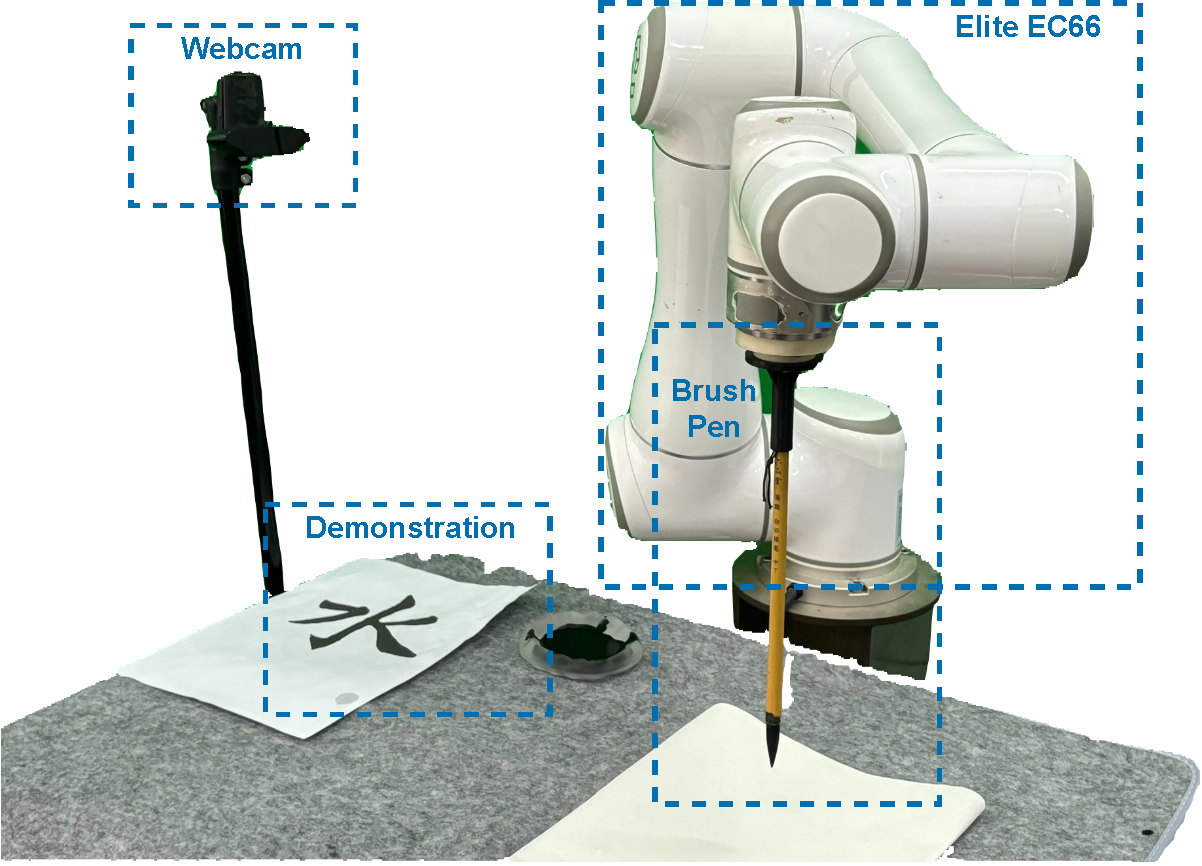
\includegraphics[width=3in]{./fig/fig8a.pdf}
    }
    \subfloat[]{
        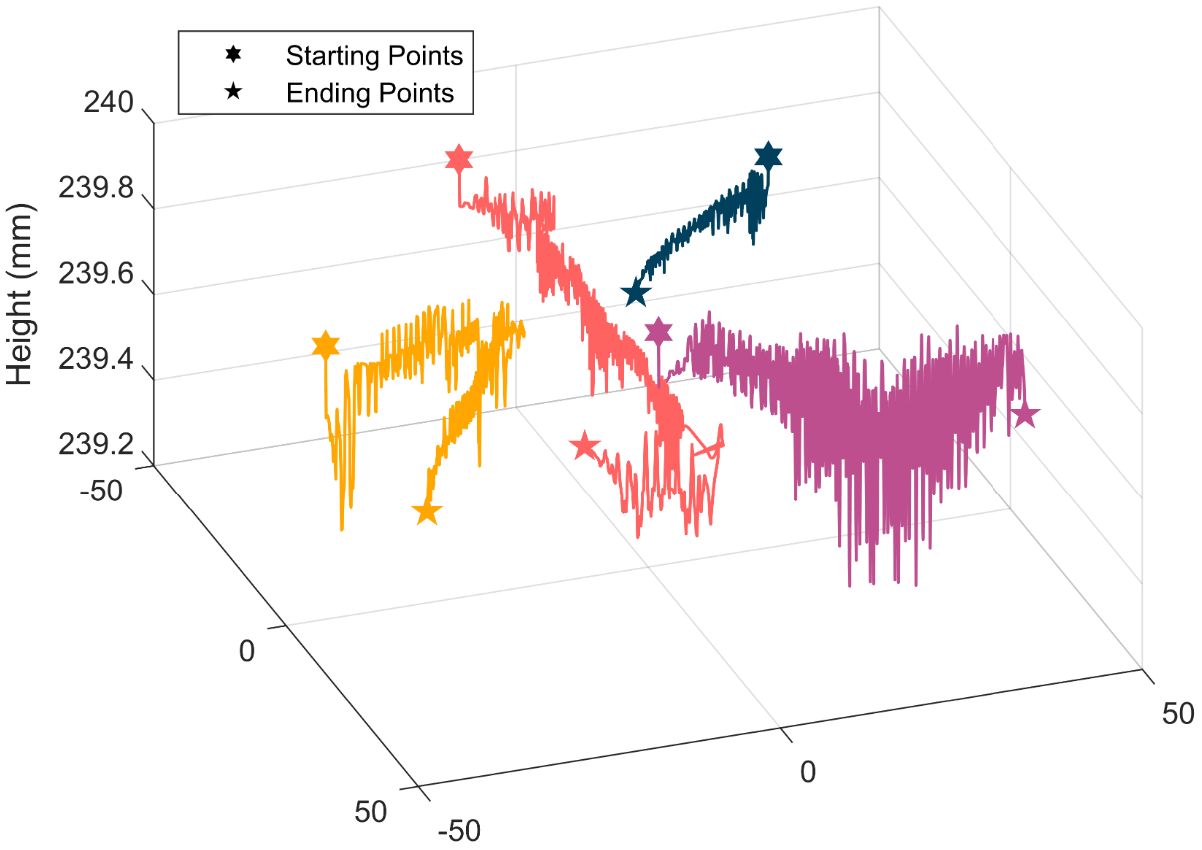
\includegraphics[width=3in]{./fig/fig8b.pdf}
    }
    \quad
    \subfloat[]{
        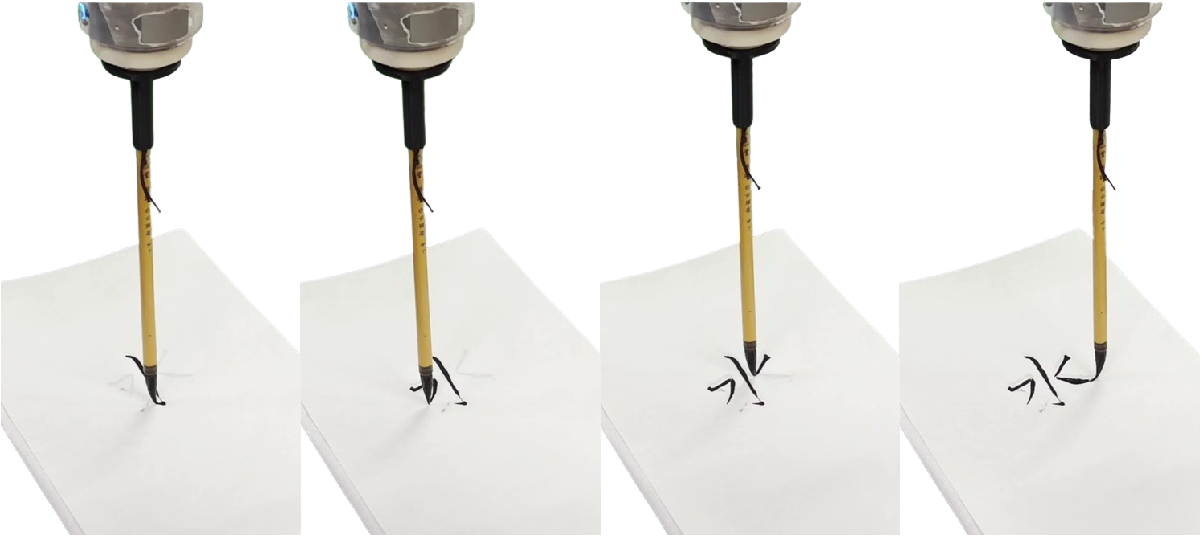
\includegraphics[width=4in]{./fig/fig8g.pdf}
    }
    \subfloat[]{
        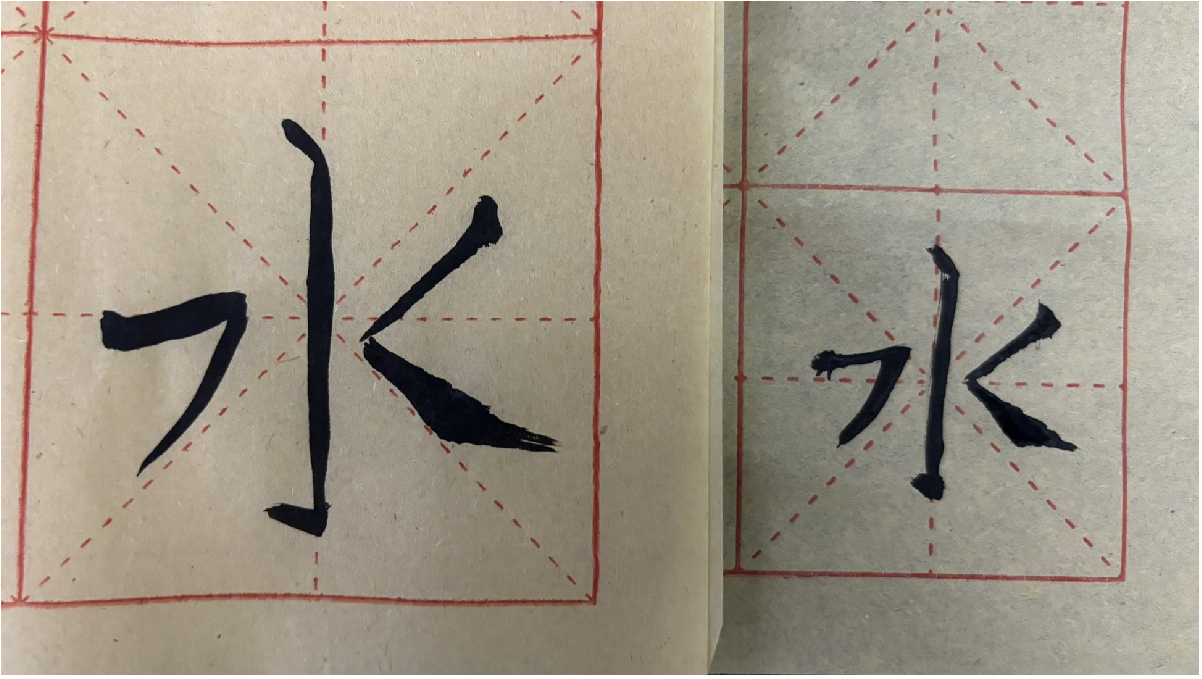
\includegraphics[width=2in]{./fig/fig9.pdf}
    }
    \caption{The real-world experiments. (a) The setup of the experiment platform. (b) The motion of the writing task (c) The experiment result of writing a Chinese character with the brush pen (d) Comparison of the experiment results writing on different sizes of paper.}
    \label{fig8}
\end{figure*}

\section{Conclusion}
We introduce an image-based imitation learning framework for robotic writing, specifically for traditional Chinese calligraphy. The framework leverages the FGMM for time encoding and deviation analysis to capture intricate stroke features. Through simulations and real-world experiments with a brush pen, the approach presents the improvement of skill transfer and generalization across various paper sizes. 

However, the capability of the writing skill mapping to the real space requires further enhancement. In future work, we will incorporate visual feedback to further control the reproduction of writing skills in the real world.

\bibliographystyle{IEEEtran}
\bibliography{IEEEabrv,reference.bib}
\end{document}
